% Preamble
\documentclass{article}


% Package Imports
\usepackage{../../../../mypackages}

% Macros
\usepackage{../../../../mymacros}

% Homework Details and Basic Document Settings
\pagestyle{fancy}
\lhead{\textbf{Eric Xia}}
\chead{MATH134 (Professor Ebru Bekyel): Week 1 Assignment}
\cfoot{\thepage}

\renewcommand\headrulewidth{0.4pt}
\renewcommand\footrulewidth{0.4pt}

\setlength\parindent{0pt}


% Title Page
\title{
    \vspace{2in}
    \textmd{\textbf{MATH134: Week 1 Assignment}}\\
    \normalsize\vspace{0.1in}\small{Due on October 5, 2020 at 5:45 PM}\\
    \vspace{0.1in}\large{\textit{Professor Ebru Bekyel}}
    \vspace{3in}
}

\author{\textbf{Eric Xia}}
\date{}


% Problem Headers and Footers
\fancypagestyle{page2}{\rhead{Section 1.2 Problem 70}\fancyfoot[L]{Section 1.2 Problem 74 continued on next page \ldots}}
\fancypagestyle{page3}{\rhead{Section 1.2 Problem 74}}
\fancypagestyle{page4}{\rhead{Section 1.3 Problem 58}\fancyfoot[L]{Section 1.4 Problem 52 continued on next page \ldots}}
\fancypagestyle{page5}{\rhead{Section 1.4 Problem 52}}
\fancypagestyle{page6}{\rhead{Section 1.8 Problem 6}\fancyfoot[L]{Section 1.8 Problem 6 continued on next page \ldots}}
\fancypagestyle{page7}{\rhead{Section 1.8 Problem 6}}


%-------------------------------------------------------------------------------------------------------------------------------------------------------------------------------------------------------------------------
%-------------------------------------------------------------------------------------------------------------------------------------------------------------------------------------------------------------------------
%-------------------------------------------------------------------------------------------------------------------------------------------------------------------------------------------------------------------------
\begin{document}

    \maketitle
    \pagebreak


    \thispagestyle{page2}
    \begin{tbhtheorem}{Section 1.2 Problem 70}
        Show that the sum of two rational numbers is a rational number.
    \end{tbhtheorem}

    \begin{proof}
    \noindent Let $x$ and $y$ be two rational numbers. Since $x$ is a rational number, by the definition of rational numbers, $x$ can be expressed as the fraction of two integers $p_1$ and $q_1$, where $q_1 \not = 0$:

    \begin{equation*}
        x = \frac{p_1}{q_1}
    \end{equation*}

    \noindent Similarly, $y$ can be expressed as

    \begin{equation*}
        y = \frac{p_2}{q_2}
    \end{equation*}

    \noindent where both $p_2$ and $q_2$ are integers, and $q_2 \not = 0$. Then the sum of $x$ and $y$ is given by

    \begin{align*}
        x + y   &= \frac{p_1}{q_1} + \frac{p_2}{q_2} \\
                &= \frac{p_1}{q_1}\cdot \frac{q_2}{q_2} + \frac{p_2}{q_2} \cdot \frac{q_1}{q_1} \\
                &= \frac{p_1 q_2 + p_2 q_1}{q_1 q_2}
    \end{align*}

    \noindent Because $p_1,q_1,p_2$ and $q_2$ are all integers, where $q_1,q_2 \not = 0$, and integers are closed under multiplication and addition, therefore

    \[
        p_1 q_2 + p_2 q_1
    \]

    \noindent is also an integer and

    \[
        q_1 q_2
    \]

    \noindent is a nonzero integer. Because $x+y$ can be expressed as an integer divided by a nonzero integer, then by the definition of a rational number, $x+y$ is also a rational number. \\
    \end{proof}



    \begin{tbhtheorem}{Section 1.2 Problem 71}
        Show that the sum of a rational number and an irrational number is irrational.
    \end{tbhtheorem}

    \begin{proof}
    \noindent Let $x$ be a rational number and $y$ be an irrational number, and let $z=x+y$. Suppose that $z$ is a rational number, hence $z$ can be expressed as

    \begin{align*}
        z            &= x + y \\
        \therefore y &= z + (-x)
    \end{align*}

    \noindent Because $x$ is a rational number and $-x=-1\cdot x$, where 1 is an integer and $x$ is a rational number, therefore $-x$ is also a rational number. Since $z$ is a rational number, therefore

    \[
        y = z + (-x)
    \]

    \noindent is also a rational number because rational numbers are closed under addition. This is proved for  Section 1.2 Problem 70, listed above this proof. The assumption that $x+y=z$, where $z$ is a rational number
    has led to a contradiction. We can conclude therefore that the expression $x+y$ must have an irrational value.

    \end{proof}



    \begin{tbhtheorem}{Section 1.2 Problem 74}
        Show by example that the sum of two irrational numbers (a) can be rational; (b) can be irrational. Do the same for the product of two irrational numbers.
    \end{tbhtheorem}

     Let $x$ and $y$ be two irrational numbers, and let $S=x+y$ and $P=xy$. Suppose that $x=5 + 2\sqrt{13}$ and $y=-2\sqrt{13}$. Then

        \begin{align*}
            S   &= x + y \\
                &= (5+2\sqrt{13}) + (-2\sqrt{13}) \\
                &= 5
        \end{align*}

        \noindent Here, $S$ is rational. Now suppose that $x=5\sqrt{7}$ and $y=13\sqrt{17}$. Then

        \begin{align*}
            S   &= x + y \\
                &= (5\sqrt{7}) + (13\sqrt{17}) \\
                &= 5\sqrt{7} + 13\sqrt{17}
        \end{align*}

        \noindent Here, $S$ is irrational. Hence, $x+y$ can be both rational and irrational.

        Suppose that $x=\sqrt{3}$ and $y=\sqrt{7}$. Then

        \begin{align*}
            P   &= xy \\
                &= \sqrt{3} \cdot \sqrt{7} \\
                &= \sqrt{21}
        \end{align*}

        \noindent Here, $P$ is irrational. Now suppose that $x=\sqrt{2}$ and $y=\sqrt{18}$. Then

        \begin{align*}
            P   &= xy \\
                &= \sqrt{2} \cdot \sqrt{18} \\
                &= \sqrt{36} \\
                &= 6
        \end{align*}

        \noindent Here, $P$ is rational. Therefore, $xy$ can be both rational and irrational.



    \thispagestyle{page3}

    \begin{tbhtheorem}{Section 1.3 Problem 53}
        Show that
        \[
            \big| |a| - |b|\big|\leq |a-b| \forall a,b,\in\mathbb{R}
        \]
    \end{tbhtheorem}

    \begin{proof}
        Because both $\big |a|-|b|\big|\geq 0$ and $|a-b|\geq 0$,

        \[
            \big| |a|-|b|\big|^2 \leq |a-b|^2
        \]

        Because both $\big| |a|-|b|\big|^2\geq 0$ and $|a-b|^2\geq 0$, we can remove the outside absolute value signs such that

        \begin{align*}
            \left(|a|-|b|\right)^2 \leq (a-b)^2 \\
            |a|^2 - 2|a||b| + |b|^2 \leq a^2 - 2ab + b^2
        \end{align*}

        Because $|a|^2\geq 0$ and $|b|^2\geq 0$, we can remove the absolute value signs from $|a|^2$ and $|b|^2$. Then we have

        \begin{align*}
            \cancel{a^2} - \cancel{2}|a||b| + \cancel{b^2}   & \leq \cancel{a^2} -\cancel{2}ab + \cancel{b^2} \\
            -|a||b|                                          & \leq ab
        \end{align*}

        \begin{align*}
            \text{For }
            \begin{cases}
                a=0 \text{ and } b=0,       & -|a||b| = ab \\
                a<0 \text{ or }  b<0,       & -|a||b| \leq ab \\
                a<0 \text{ and } b<0,       & -|a||b| < ab \\
                a>0 \text{ or }  b>0,       & -|a||b| \leq ab \\
                a>0 \text{ and } b>0,       & -|a||b| < ab
            \end{cases}
        \end{align*}

        Then it is true that

        \[
            -|a||b| \leq ab
        \]

        and hence

        \[
            \big| |a| - |b|\big|\leq |a-b| \forall a,b,\in\mathbb{R}
        \]


    \end{proof}



    \pagebreak
    \thispagestyle{page4}

    \begin{tbhtheorem}{Section 1.3 Problem 58}
        Given that $0\leq a\leq b$, show that
        \begin{equation*}
            a \leq \sqrt{ab} \leq \frac{a+b}{2} \leq b.
        \end{equation*}
    \end{tbhtheorem}

    \begin{proof}

        Given

        \[
            a \leq b, a\geq 0,
        \]

        \noindent then

        \begin{align*}
            a^2  & \leq ab \\
            a    & \leq \sqrt{ab}
        \end{align*}

        \noindent Suppose that

        \begin{align*}
            \sqrt{ab} \leq \frac{a+b}{2} \iff ab  &   \leq \left(\frac{a+b}{2}\right)^2 \\
            ab  &   \leq \frac{(a+b)^2}{4} \\
            4ab &   \leq a^2 + 2ab + b^2 \\
            0   &   \leq a^2 - 2ab + b^2 \\
            0   &   \leq (a-b)^2
        \end{align*}

        \noindent Because any real number squared has a nonnegative value, thus it is true that

        \[
            0 \leq (a-b)^2
        \]

        \noindent and so

        \[
            \sqrt{ab} \leq \frac{a+b}{2}
        \]

        \noindent Recall that

        \begin{align*}
            a             & \leq  b \\
            a + b         & \leq  2b \\
            \frac{a+b}{2} & \leq b
        \end{align*}

        \noindent Hence,

        \[
            a \leq \sqrt{ab} \leq \frac{a+b}{2} \leq b
        \]

    \end{proof}


    \begin{tbhtheorem}{Section 1.4 Problem 52}
        The perpendicular bisector of the line segment $\overline{PQ}$ is the line which is perpendicular to $\overline{PQ}$ and passes through the midpoint of $\overline{PQ}$. Find an equation for the
        perpendicular bisector of the line segment that joins points $P(-1,3)$ and $Q(3,-4)$.
    \end{tbhtheorem}

    \noindent The midpoint, $M$, of the line segment $\overline{PQ}$ is given by

    \begin{align*}
        M &= \left(\frac{-1+3}{2}, \frac{-4+3}{2} \right) \\
          &= \left(1, -\frac{1}{2}\right)
    \end{align*}

    \noindent The slope, $m$, of the line segment $\overline{PQ}$ is given by

    \begin{align*}
        m   &=  \frac{-4-3}{3-(-1)} \\
            &= -\frac{7}{4}
    \end{align*}

    \pagebreak
    \thispagestyle{page5}

    \noindent The opposite of the reciprocal of $-\frac{7}{4}$ is $\frac{4}{7}$, and so the slope of the perpendicular bisector of $\overline{PQ}$ is also $\frac{4}{7}$. An equation for this perpendicular bisector
    could be written as

    \[
        y + \frac{1}{2} = \frac{4}{7} \left(x - 1\right)
    \]



    \begin{tbhtheorem}{Section 1.7 Problem 59}
        Show that every function defined for all real numbers can be written as the sum of an even function and an odd function.
    \end{tbhtheorem}

    \begin{proof}
        Suppose

        \[
            f(x) = e(x) + o(x),
        \]

        \noindent where $e(x)$ is an even function and $o(x)$ is an odd function, both of which are defined for all real numbers. By the definitions of even and odd functions, we also have

        \begin{align*}
            f(-x)   &= e(-x) + o(-x) \\
                    &= e(x) - o(x)
        \end{align*}

        \noindent Solving the following system of equations,

        \begin{align*}
            \begin{cases}
                f(x) &= e(x) + o(x) \\
                f(-x) &= e(x) - o(x)
            \end{cases}
        \end{align*}

        \noindent it follows that we can express $e(x)$ and $o(x)$ in terms of $f(x)$:

        \begin{align*}
            2e(x) &= f(x) + f(-x) \\
            e(x)  &= \frac{f(x) + f(-x)}{2} \\
            2o(x) &= f(x) - f(-x) \\
            o(x)  &= \frac{f(x)-f(-x)}{2}
        \end{align*}

        \noindent Suppose $e(-x)=e(x)$. Then

        \begin{align*}
            e(-x)                       &=  e(x) \\
            \frac{f(-x)+f(-(-x))}{2}    &= \frac{f(x)+f(-x)}{2} \\
            \frac{f(-x)+f(x)}{2}       &= \frac{f(x)+f(-x)}{2}
        \end{align*}

        \noindent Thus, by the definition of even functions, $e(x)$ is an even function. Now suppose $o(-x)=-o(x)$. Then

        \begin{align*}
            o(-x)                       &= -o(x) \\
            \frac{f(-x)-f(-(-x))}{2}    &= -\frac{f(x)-f(-x)}{2} \\
            \frac{f(-x)-f(x)}{2}        &= \frac{f(-x)-f(x)}{2} \\
        \end{align*}

        \noindent Thus, by the definition of an odd function, $o(x)$ is an odd function. Again, suppose

        \begin{align*}
            f(x)    &= e(x) + o(x) \\
                    &= \frac{f(x)+f(-x)}{2} + \frac{f(x)-f(-x)}{2} \\
                    &= \frac{2f(x)}{2} \\
                    &= f(x)
        \end{align*}

        \noindent Hence, a function defined for all real numbers can be written as the sum of an even function and an odd function.

    \end{proof}

    \pagebreak
    \thispagestyle{page6}



    \begin{tbhtheorem}{Section 1.8 Problem 6}
        Show that the statement \\
        \begin{equation*}
            1^3 + 2^3 + 3^3 +\dots + n^3 = \left(1+2+3+\dots+n\right)^2
        \end{equation*}
        holds for all positive integers n.
    \end{tbhtheorem}

    \noindent Before the proof for this statement, below first is a proof that

    \[
        1 + 2 + 3 + \dots + n = \frac{n(n+1)}{2} \forall n\in\mathbb{Z}^+
    \]

    \noindent which will be implemented in the proof for the current problem: \\

    \begin{tcolorbox}[colback = red!10]

        \begin{proof}
        \noindent Let $S$ be the set of positive integers $n$ for which

        \begin{equation*}
            1 + 2 + 3 + \dots + n = \frac{n(n+1)}{2}
        \end{equation*}

        \noindent Then $1\in S$ since
        \begin{equation*}
            1 = \frac{1(1+1)}{2}
        \end{equation*}

        \noindent Assume that $k\in S$; that is, assume that

        \begin{equation*}
            1 + 2 + 3 \dots + k = \frac{k(k+1)}{2}
        \end{equation*}

        \noindent Adding up the first $k+1$ integers, we have

        \begin{align*}
            1 + 2 + 3 + \dots + k + (k+1)   &= [1+2+3+\dots+k] + (k+1) \\
            &= \frac{k(k+1)}{2} + (k+1), \text{ by the induction hypothesis} \\
            &= \frac{k(k+1)+2(k+1)}{2} \\
            &= \frac{(k+1)(k+2)}{2}
        \end{align*}

        \noindent and so $k+1\in S$. Thus, by the principle of induction, we can conclude that all positive integers are in $S$; that is, we can conclude that

        \begin{equation*}
            1 + 2 + 3 + \dots + n = \frac{n(n+1)}{2} \forall n \in \mathbb{Z}^+
        \end{equation*}

        \end{proof}
    \end{tcolorbox}

    \noindent Having proved the above statement, we will now begin proving the actual Section 1.8 Problem 6:

    \begin{proof}

        Let $S$ be the set of positive integers $n$ for which

        \[
            1^3 + 2^3 + 3^3 + \dots + n^3 = (1+2+3+\dots +n)^2
        \]

        \noindent Then $1\in S$ since

        \[
            1^3 = 1^2
        \]

        \noindent Assume that $k\in S$; that is, assume that

        \[
            1^3 + 2^3 + 3^3 + \dots + k^3 = (1+2+3+\dots + k)^2
        \]

        \noindent Summing up the cubes of the first $k+1$ integers, we have

        \begin{align*}
            1^3 + 2^3 + 3^3 + k^3 + (k+1)^3     &= [1^3 +2^3 +3^3 +\dots +k^3] + (k+1)^3 \\
                                                &= (1+2+3+\dots +k)^2 + (k+1)^3 \\
                                                &= \left(\frac{k(k+1)}{2}\right)^2 + (k+1)^3 \\
                                                &= \frac{k^2 (k+1)^2}{4} + (k+1)^3 \\
                                                &= \frac{k^2 (k+1)^2}{4} + \frac{4(k+1)^3}{4} \\
                                                &= \frac{k^2 (k+1)^2 + 4(k+1)^2 (k+1)}{4} \\
                                                &= \frac{(k+1)^2 (k^2 +4(k+1))}{4}
        \end{align*}

        \pagebreak

        \begin{align*}
            \color{white} 1^3 + 2^3 + 3^3 + k^3           \color{black} &= \frac{(k+1)^2 (k^2 + 4k + 4)}{4} \\
                                                                        &= \frac{(k+1)^2 (k+2)^2}{4} \\
                                                                        &= \left(\frac{(k+1)(k+2)}{2} \right)^2 \\
                                                                        &= (1+2+3+\dots + (k+1))^2
        \end{align*}

        \noindent Therefore, by the principle of mathematical induction, we can conclude that all positive integers are in $S$; that is, we can conclude that

        \[
            1^3 + 2^3 + 3^3 + \dots + n^3 = (1+2+3+ \dots + n)^2, \forall n\in \mathbb{Z}^+
        \]


    \end{proof}


    \thispagestyle{page7}


    \begin{tbhtheorem}{Section 1.8 Problem 18}
        Show that, given a unit length, for each positive integer $n$, a line segment of length $\sqrt{n}$ can be constructed by straight edge and compass.
    \end{tbhtheorem}

    \begin{proof}

        Let set $S$ be composed of positive integers $n$ for which a line segment of length $\sqrt{n}$ can be constructed by straight edge and compass. Then $1\in S$ because $\sqrt{1}=1$, hence a line segment of length
        $\sqrt{1}$ can be directly constructed by straight edge. Assume that $k\in S$; that is,
        assume that a right triangle $\Delta ABC$ with legs of length $1$ and $\sqrt{k}$ can be constructed, using the compass to make the right angle, like so:

        \begin{center}
            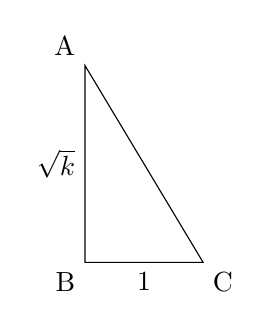
\begin{tikzpicture}[scale=0.5]
                \coordinate[label=above left:A] (A) at (0,5);
                \coordinate[label=below left:B] (B) at (0,0);
                \coordinate[label=below right:C] (C) at (3,0);
                \draw (A) -- (B) node [midway, left] {$\sqrt{k}$} -- (C) node [midway, below] {1} -- cycle;
                \tkzMarkRightAngle [size=0.5](A,B,C)
            \end{tikzpicture}
        \end{center}

        \noindent By the Pythagorean Theorem, the hypotenuse of $\Delta ABC$ is $\sqrt{k+1}$, as depicted in the below figure.

        \begin{center}
            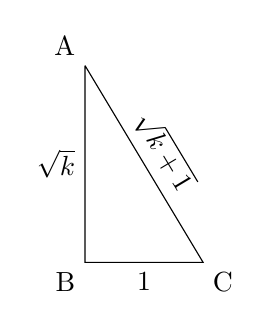
\begin{tikzpicture}[scale=0.5]
                \coordinate[label=above left:A] (A) at (0,5);
                \coordinate[label=below left:B] (B) at (0,0);
                \coordinate[label=below right:C] (C) at (3,0);
                \draw (A) -- (B) node [midway, left] {$\sqrt{k}$} -- (C) node [midway, below] {1} -- (A) node [midway, sloped, above] {$\sqrt{k+1}$};
                \tkzMarkRightAngle [size=0.5](A,B,C)
            \end{tikzpicture}
        \end{center}

        \noindent By the induction hypothesis, we can construct a right triangle using a compass and straightedge with legs of length 1 and $\sqrt{k+1}$. We can do this by constructing a ray $\overrightarrow{CD}$ of
        length 1 and angle measure $\angle ACB + 270\degree$ and connect points $A$ and $D$, thus forming a triangle $\Delta ACD$ with legs of length 1 and $\sqrt{k+1}$. Again by the Pythagorean Theorem, the hypotenuse of
        $\Delta ACD$ is of length $\sqrt{(k+1)+1}=\sqrt{k+2}$.

        \begin{center}
            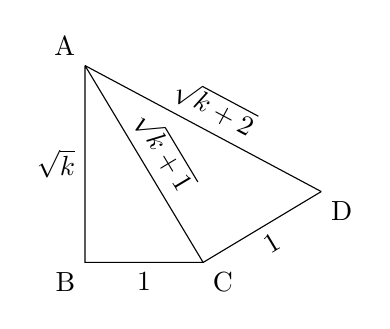
\begin{tikzpicture}[scale=0.5]
                \coordinate[label=above left:A] (A) at (0,5);
                \coordinate[label=below left:B] (B) at (0,0);
                \coordinate[label=below right:C] (C) at (3,0);
                \coordinate[label=below right:D] (D) at (6,1.8);
                \draw (A) -- (B) node [midway, left] {$\sqrt{k}$} -- (C) node [midway, below] {1} -- (A) node [midway, sloped, above] {$\sqrt{k+1}$};
                \draw (C) -- (D) node [midway, sloped, below] {1};
                \draw (D) -- (A) node [midway, sloped, above] {$\sqrt{k+2}$};
                \tkzMarkRightAngle [size=0.5](A,B,C)
                \tkzMarkRightAngle [size=0.5](A,C,D)
            \end{tikzpicture}
        \end{center}

        \noindent Because the line segment $\overline{AD}$ of length $\sqrt{k+2}$ was constructed by straight edge and compass using the line segment $\overline{AD}$ of length $\sqrt{k+1}$ as a reference, thus
        $k+1\in S$. \\

        \noindent Hence, by the axiom of induction, we can conclude that all positive integers are in $S$; that is, we can conclude that, given a unit length, for each positive integer $n$, a line segment of length
        $\sqrt{n}$ can be constructed by straight edge and compass.


    \end{proof}


\end{document}